\documentclass{standalone}
\usepackage{tikz}
\usetikzlibrary{patterns, positioning}
\usepackage[sfdefault]{ClearSans} %% option 'sfdefault' activates Clear Sans as the default text font
\usepackage[T1]{fontenc}

\begin{document}
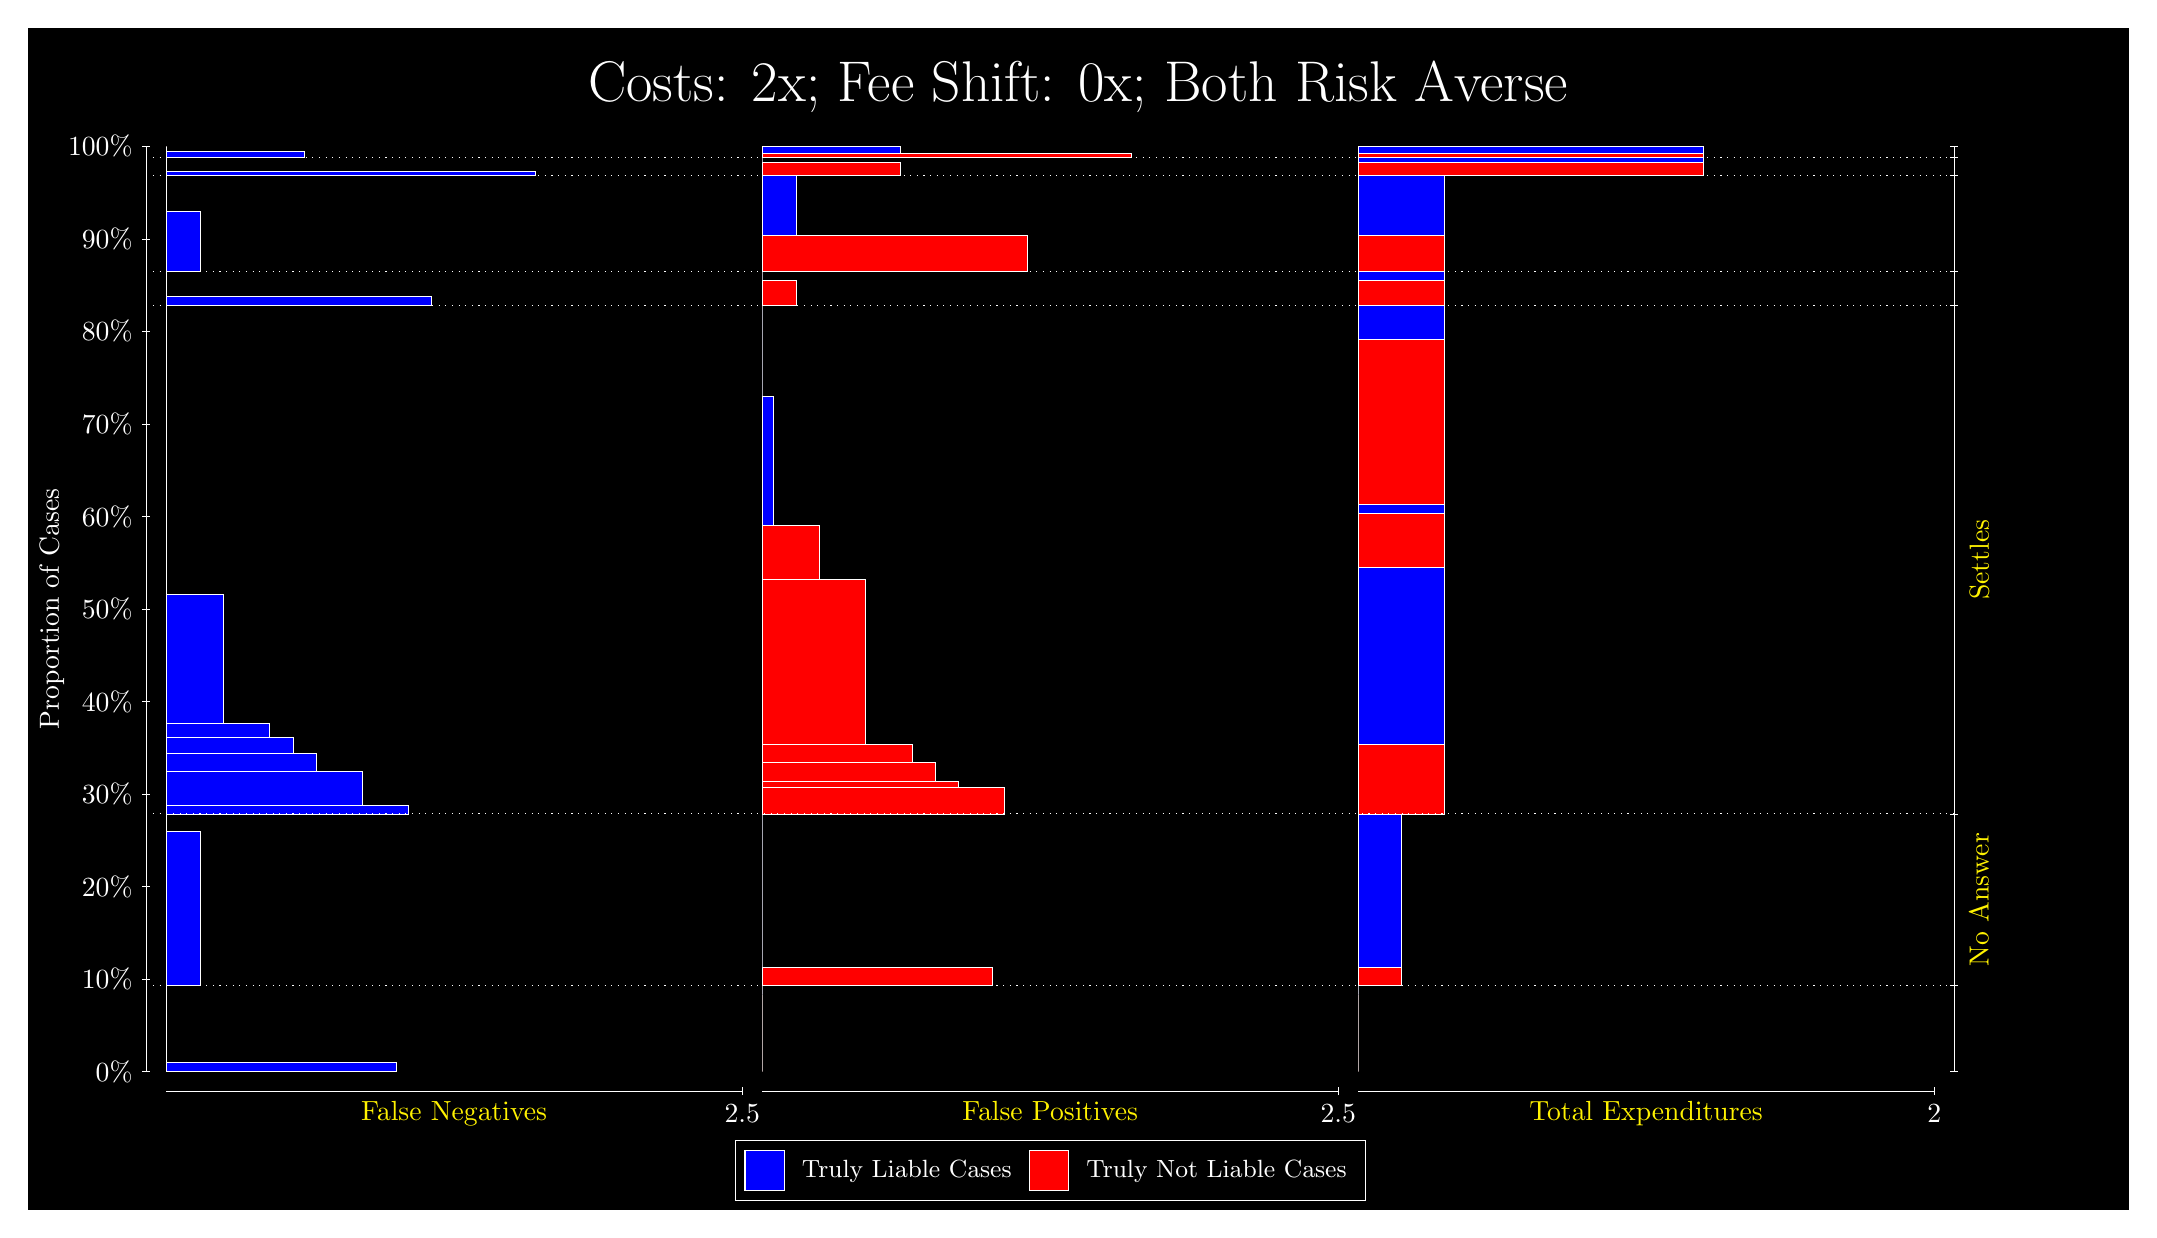
\begin{tikzpicture}
\draw[fill=black] (0,0) rectangle (26.667,15);
\draw[text=white] (0,13.5) rectangle (26.667,15) node[midway] {\huge Costs: 2x; Fee Shift: 0x; Both Risk Averse};
\draw[white, very thin] (1.5,1.75) -- (1.5,13.5);
\node[rotate=90, text=white, anchor=center] at (0.3, 7.625) {Proportion of Cases};
\draw[white, very thin] (1.45,1.75) -- (1.55,1.75);
\node[text=white, anchor=east] at (1.45, 1.75) {0\%};
\draw[white, very thin] (1.45,2.925) -- (1.55,2.925);
\node[text=white, anchor=east] at (1.45, 2.925) {10\%};
\draw[white, very thin] (1.45,4.1) -- (1.55,4.1);
\node[text=white, anchor=east] at (1.45, 4.1) {20\%};
\draw[white, very thin] (1.45,5.275) -- (1.55,5.275);
\node[text=white, anchor=east] at (1.45, 5.275) {30\%};
\draw[white, very thin] (1.45,6.45) -- (1.55,6.45);
\node[text=white, anchor=east] at (1.45, 6.45) {40\%};
\draw[white, very thin] (1.45,7.625) -- (1.55,7.625);
\node[text=white, anchor=east] at (1.45, 7.625) {50\%};
\draw[white, very thin] (1.45,8.8) -- (1.55,8.8);
\node[text=white, anchor=east] at (1.45, 8.8) {60\%};
\draw[white, very thin] (1.45,9.975) -- (1.55,9.975);
\node[text=white, anchor=east] at (1.45, 9.975) {70\%};
\draw[white, very thin] (1.45,11.15) -- (1.55,11.15);
\node[text=white, anchor=east] at (1.45, 11.15) {80\%};
\draw[white, very thin] (1.45,12.325) -- (1.55,12.325);
\node[text=white, anchor=east] at (1.45, 12.325) {90\%};
\draw[white, very thin] (1.45,13.5) -- (1.55,13.5);
\node[text=white, anchor=east] at (1.45, 13.5) {100\%};

\draw[white, very thin] (24.457,1.75) -- (24.457,13.5);
\draw[white, very thin] (24.407,1.75) -- (24.507,1.75);
\node[anchor=west] at (24.407, 1.75) {};
\draw[white, very thin] (24.407,2.8432) -- (24.507,2.8432);
\node[anchor=west] at (24.407, 2.8432) {};
\draw[white, very thin] (24.407,5.0214) -- (24.507,5.0214);
\node[anchor=west] at (24.407, 5.0214) {};
\draw[white, very thin] (24.407,11.478) -- (24.507,11.478);
\node[anchor=west] at (24.407, 11.478) {};
\draw[white, very thin] (24.407,11.915) -- (24.507,11.915);
\node[anchor=west] at (24.407, 11.915) {};
\draw[white, very thin] (24.407,13.129) -- (24.507,13.129);
\node[anchor=west] at (24.407, 13.129) {};
\draw[white, very thin] (24.407,13.355) -- (24.507,13.355);
\node[anchor=west] at (24.407, 13.355) {};
\draw[white, very thin] (24.407,13.5) -- (24.507,13.5);
\node[anchor=west] at (24.407, 13.5) {};

\draw[white, very thin, fill=blue] (1.75,1.75) rectangle (4.6775,1.865);
\draw[white, very thin, fill=red] (1.75,1.865) rectangle (1.75,2.8432);
\draw[white, very thin, fill=blue] (1.75,2.8432) rectangle (2.1891,4.7954);
\draw[white, very thin, fill=red] (1.75,4.7954) rectangle (1.75,5.0214);
\draw[white, very thin, fill=blue] (1.75,5.0214) rectangle (4.8239,5.1315);
\draw[white, very thin, fill=blue] (1.75,5.1315) rectangle (4.2384,5.5644);
\draw[white, very thin, fill=blue] (1.75,5.5644) rectangle (3.6529,5.7868);
\draw[white, very thin, fill=blue] (1.75,5.7868) rectangle (3.3602,5.9902);
\draw[white, very thin, fill=blue] (1.75,5.9902) rectangle (3.0674,6.1779);
\draw[white, very thin, fill=blue] (1.75,6.1779) rectangle (2.4819,7.8077);
\draw[white, very thin, fill=red] (1.75,7.8077) rectangle (1.75,11.478);
\draw[white, very thin, fill=blue] (1.75,11.478) rectangle (5.1167,11.591);
\draw[white, very thin, fill=red] (1.75,11.591) rectangle (1.75,11.915);
\draw[white, very thin, fill=blue] (1.75,11.915) rectangle (2.1891,12.678);
\draw[white, very thin, fill=red] (1.75,12.678) rectangle (1.75,13.129);
\draw[white, very thin, fill=blue] (1.75,13.129) rectangle (6.4341,13.188);
\draw[white, very thin, fill=red] (1.75,13.188) rectangle (1.75,13.355);
\draw[white, very thin, fill=blue] (1.75,13.355) rectangle (3.5065,13.441);
\draw[white, very thin, fill=red] (1.75,13.441) rectangle (1.75,13.5);
\draw[white, very thin, fill=red] (9.3189,1.75) rectangle (9.3189,2.7282);
\draw[white, very thin, fill=blue] (9.3189,2.7282) rectangle (9.3189,2.8432);
\draw[white, very thin, fill=red] (9.3189,2.8432) rectangle (12.246,3.0692);
\draw[white, very thin, fill=blue] (9.3189,3.0692) rectangle (9.3189,5.0214);
\draw[white, very thin, fill=red] (9.3189,5.0214) rectangle (12.393,5.3555);
\draw[white, very thin, fill=red] (9.3189,5.3555) rectangle (11.807,5.4405);
\draw[white, very thin, fill=red] (9.3189,5.4405) rectangle (11.515,5.6823);
\draw[white, very thin, fill=red] (9.3189,5.6823) rectangle (11.222,5.9047);
\draw[white, very thin, fill=red] (9.3189,5.9047) rectangle (10.636,7.9957);
\draw[white, very thin, fill=red] (9.3189,7.9957) rectangle (10.051,8.6913);
\draw[white, very thin, fill=blue] (9.3189,8.6913) rectangle (9.4652,10.321);
\draw[white, very thin, fill=blue] (9.3189,10.321) rectangle (9.3189,11.478);
\draw[white, very thin, fill=red] (9.3189,11.478) rectangle (9.758,11.801);
\draw[white, very thin, fill=blue] (9.3189,11.801) rectangle (9.3189,11.915);
\draw[white, very thin, fill=red] (9.3189,11.915) rectangle (12.686,12.366);
\draw[white, very thin, fill=blue] (9.3189,12.366) rectangle (9.758,13.129);
\draw[white, very thin, fill=red] (9.3189,13.129) rectangle (11.075,13.297);
\draw[white, very thin, fill=blue] (9.3189,13.297) rectangle (9.3189,13.355);
\draw[white, very thin, fill=red] (9.3189,13.355) rectangle (14.003,13.414);
\draw[white, very thin, fill=blue] (9.3189,13.414) rectangle (11.075,13.5);
\draw[white, very thin, fill=red] (16.888,1.75) rectangle (16.888,2.7282);
\draw[white, very thin, fill=blue] (16.888,2.7282) rectangle (16.888,2.8432);
\draw[white, very thin, fill=red] (16.888,2.8432) rectangle (17.437,3.0692);
\draw[white, very thin, fill=blue] (16.888,3.0692) rectangle (17.437,5.0214);
\draw[white, very thin, fill=red] (16.888,5.0214) rectangle (17.986,5.9047);
\draw[white, very thin, fill=blue] (16.888,5.9047) rectangle (17.986,8.1481);
\draw[white, very thin, fill=red] (16.888,8.1481) rectangle (17.986,8.8436);
\draw[white, very thin, fill=blue] (16.888,8.8436) rectangle (17.986,8.9537);
\draw[white, very thin, fill=red] (16.888,8.9537) rectangle (17.986,11.045);
\draw[white, very thin, fill=blue] (16.888,11.045) rectangle (17.986,11.478);
\draw[white, very thin, fill=red] (16.888,11.478) rectangle (17.986,11.801);
\draw[white, very thin, fill=blue] (16.888,11.801) rectangle (17.986,11.915);
\draw[white, very thin, fill=red] (16.888,11.915) rectangle (17.986,12.366);
\draw[white, very thin, fill=blue] (16.888,12.366) rectangle (17.986,13.129);
\draw[white, very thin, fill=red] (16.888,13.129) rectangle (21.279,13.297);
\draw[white, very thin, fill=blue] (16.888,13.297) rectangle (21.279,13.355);
\draw[white, very thin, fill=red] (16.888,13.355) rectangle (21.279,13.414);
\draw[white, very thin, fill=blue] (16.888,13.414) rectangle (21.279,13.5);
\draw[white, dotted] (1.5,2.8432) -- (24.457,2.8432);
\draw[white, dotted] (1.5,5.0214) -- (24.457,5.0214);
\draw[white, dotted] (1.5,11.478) -- (24.457,11.478);
\draw[white, dotted] (1.5,11.915) -- (24.457,11.915);
\draw[white, dotted] (1.5,13.129) -- (24.457,13.129);
\draw[white, dotted] (1.5,13.355) -- (24.457,13.355);
\draw[white, very thin] (1.75,1.5) -- (9.0689,1.5);
\node[text=yellow, anchor=north] at (5.4094, 1.5) {False Negatives};
\draw[white, very thin] (9.0689,1.45) -- (9.0689,1.55);
\node[text=white, anchor=north] at (9.0689, 1.45) {2.5};

\draw[white, very thin] (9.3189,1.5) -- (16.638,1.5);
\node[text=yellow, anchor=north] at (12.978, 1.5) {False Positives};
\draw[white, very thin] (16.638,1.45) -- (16.638,1.55);
\node[text=white, anchor=north] at (16.638, 1.45) {2.5};

\draw[white, very thin] (16.888,1.5) -- (24.207,1.5);
\node[text=yellow, anchor=north] at (20.547, 1.5) {Total Expenditures};
\draw[white, very thin] (24.207,1.45) -- (24.207,1.55);
\node[text=white, anchor=north] at (24.207, 1.45) {2};


\node[text=yellow, centered, rotate=90] at (24.777, 3.9323) {No Answer};
\node[text=yellow, centered, rotate=90] at (24.777, 8.2495) {Settles};





\draw (12.978300999999998,1.5) node[draw=none] (baseCoordinate) {};
\begin{scope}[align=center]
        \matrix[scale=0.5, draw=white, below=0.5cm of baseCoordinate, nodes={draw}, column sep=0.1cm]{
            \node[rectangle, draw, minimum width=0.5cm, minimum height=0.5cm, fill=blue] {}; &
            \node[draw=none, font=\small, text=white] (B) {Truly Liable Cases}; &
            \node[rectangle, draw, minimum width=0.5cm, minimum height=0.5cm, fill=red] {}; &
            \node[draw=none, font=\small, text=white] (B) {Truly Not Liable Cases}; \\
            };
\end{scope}

\end{tikzpicture}
\end{document}